\section{Progettazione e Implementazione}
\label{section:progettazione}


Per favorire un modello da studiare che permetta di risolvere gli obiettivi descritti 
pocanzi sono state prese le decisioni qui di seguito elencate.

Iniziamo con il dire che il social network verrà astratto ad un grafo scale-free dove ogni 
nodo è un utente che possiede alcune caratteristiche.

Per il primo obiettivo verrà posta l'attenzione su due algoritmi, impiegati per la creazione di grafi, 
che formano modelli di rete differenti.

Inizialmente verrà fatto vedere come una notizia viene propagata in un grafo di tipo 
``Preferential Attachment'' suggerito da Barabási e Albert~\cite{biblio:barabasilab_emergence}.

Le simulazioni poi proseguiranno con un altra topologia di grafo, sempre scale-free 
con Power Law Degree, descritta però dall'algoritmo di Dorogovtsev e Mendes~\cite{biblio:evolution_networks}.

Il lavoro non parte da dati reali e la scelta di queste topologie di grafi è data 
dalla peculiarità di alcune loro caratteristiche che elencherò qui di seguito:
\begin{itemize}
 \item La topologia di grafo Preferential Attachment:
 \begin{itemize}
  \item è un modello ampiamente utilizzato per la sua semplicità;
  \item è impiegato da buona parte di studi che trattano argomenti somiglianti lo ``Spreading Rumors'';
  \item non è un grafo di tipo frattale~\cite{biblio:fractal_resistant_disease} ma ha una caratteristica simile. 
 Non possedendo cricche di almeno 3 nodi, se un nodo non condivide la notizia, 
 tutti i suoi nodi ``figli'' non riceveranno mai l'informazione.
 \end{itemize}
 
 \item La topologia di grafo definita da Dorogovtsev e Mendes invece:
  \begin{itemize}
  \item ha un modello decisamente più complesso;
  \item può avere all'interno del grafo cricche da 3 o più nodi e questo permette una probabilità maggiore di condivisione della notizia;
  \item più somigliante\footnote{\scriptsize Non esiste un modello virtuale di una rete sociale reale. 
  Tutte le ottimizzazioni che vengono apportate sono per rendere i risultati di queste simulazioni più attinenti alla realtà.}
  ad una struttura reale di rete sociale.
 \end{itemize}
\end{itemize}

Cercando di migliorare il modello totale della simulazione è stato deciso di fornire alcune proprietà alla notizia e 
agli utenti(Nodi) che compaiono nella rete sociale.

Osservando il secondo obiettivo dobbiamo fornire alla notizia un ``argomento'' e per fare ciò si 
è optato per l'inserimento di $N$ valori che definiranno quanto è adatta la notizia per ogni fascia d'età.

Avendo a disposizione la distribuzione delle età, precedentemente mostrata nel grafico di figura~\ref{img:age_distribution_social},
possiamo notare 5 intervalli di anni e quindi stabilire il valore di $N = 5$.

Dobbiamo perciò anche definire 5 gruppi di utenti per distinguere le differenti età.
Il numero di persone appartenenti ad ogni gruppo verrà semplicemente definito dalla semplice proporzione:

\[
\frac{N\_NODI\_TOTALI}{100} \cdot \%\_UTENTI\_GRUPPO
\]

%N\_NODI\_TOTALI \quad / \quad 100 \quad * \quad \%\_UTENTI\_GRUPPO
dove $\%\_UTENTI\_GRUPPO$ è la percentuale presente nel grafico di figura~\ref{img:age_distribution_social}.

A questo punto per la condivisione dell'informazione tra nodo e nodo manca solamente la formula per definire la probabilità 
della propagazione.
L'idea è quella di dare la ``possibilità'' all'utente, come nella realtà, di decidere se la 
notizia gli interessa oppure no. 
Questo ci obbliga ad aggiungere un nuovo paramentro all'utente, l'astensione alla notizia.

Così facendo la notizia verrà condivisa dall'utente \emph{'i-esimo'} con una certa età \emph{'e'} se:
\[
NOTIZIA_e \quad > \quad UTENTE_i.astensione
\]
dove $\quad NOTIZIA_e \quad$ è la forza di condivisione della notizia su una data fascia d'età \emph{'e'}, 
mentre $\quad UTENTE_i.astensione \quad$ è l'astensione alla notizia dell'utente i-esimo.

L'ultimo obiettivo agisce proprio su quest'ultima parte appena definita.
Quando si parla di ``forza della notizia'' e di ``forza di astensione'' vogliamo considerare un numero tra 0 e 1.
Per avere una probabilità di condivisione più o meno alta andremo ad agire solo sulla ``forza di astensione''.
Per come abbiamo definito la formula della condivisione basterà che la distribuzione dell'astensione sia più 
tendente a 0 per avere una miglior condivisione, o viceversa, più tendente a 1 per avere una peggior
condivisione.

\subsection{Strumenti}


Dopo aver discusso di tutte le fasi della progettazione possiamo passare all'imple-mentazione.

Le simulazioni previste saranno sviluppate in NetLogo che fornisce un ambiente semplice e piuttosto 
personalizzabile dove si possono condurre studi in parecchi campi.
NetLogo è uno strumento di sviluppo per una programmazione basata ad agenti.
Nel lavoro qui presentato gli agenti in questione saranno gli utenti della rete sociale.
Esistono molti altri simulatori di reti che prevedono una programmazione ad agenti, ma NetLogo
ha risposto brillantemente alle esigenze implementative avendo una sintassi semplice e una moltitudine di
API\footnote{\scriptsize Application Programming Interface: un insieme di funzionalità utilizzabili dal programmatore
}~\cite{biblio:netlogo_dictionary} fornite dal linguaggio stesso. 
E' stato anche scelto per la facilità con cui si riesce a modellare una 
interfaccia grafica\footnote{\scriptsize Dall’inglese GUI ovvero Graphical User Interface}.



\subsection{Topologie dei grafi}
\label{section:graph_topologies}


Come già annunciato all'inizio di questo capitolo i modelli di grafo che verranno studiati in questo lavoro
sono due.


\subsubsection{Preferential Attachment}
\label{section:graph_topologies_pa}
Il modello Preferential Attachment, come già comunicato a inizio capitolo, è altamente diffuso e conosciuto.
Tanto da avere una propria API per la creazione nel dizionario di NetLogo. 

Invocando la funzione:
\begin{lstlisting}[label=some-code, style=custom_code]
 generate-preferential-attachment turtles links num-nodes
\end{lstlisting}

che risiede all'interno dell'estensione ``network'' verrà creato un grafo di \emph{num-nodes} nodi con le proprietà 
del grafo Preferential Attachment. L'algoritmo di PA implementato in NetLogo crea per ogni nuovo nodo un solo collegamento. \\
In figura \ref{img:preferential_attachment} è presente una rappresentazione grafica di un grafo con 20 nodi.

\begin{figure}[!ht]
 \centerline{
  \begin{subfigure}[b]{0.4\textwidth}
    \begin{center}
      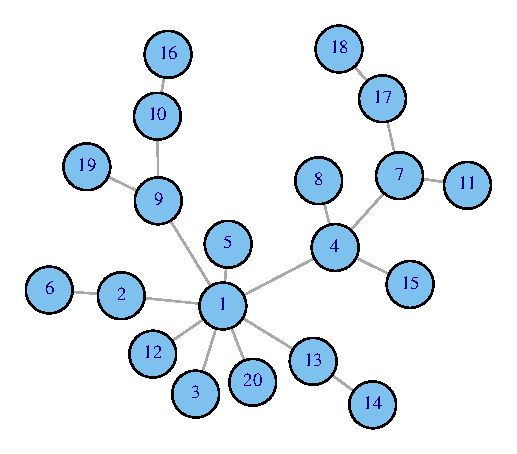
\includegraphics[width=0.75\textwidth]{img/preferential-attachment-graph.eps}
    \end{center}
    \caption{Preferential Attachment}
    \label{img:preferential_attachment}
  \end{subfigure}
  \qquad
  \qquad
  \qquad
  \begin{subfigure}[b]{0.4\textwidth}
    \begin{center}
      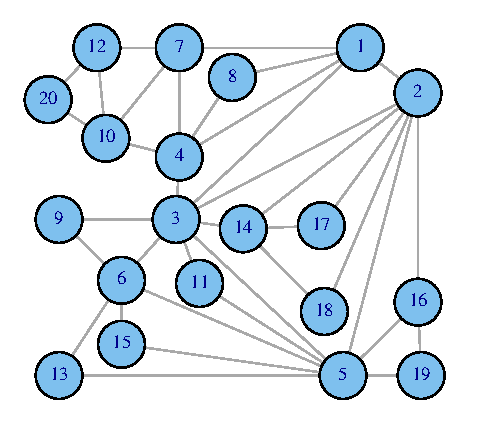
\includegraphics[width=0.75\textwidth]{img/dorogovtsev-mendes-graph.eps}
    \end{center}
    \caption{Dorogovtsev e Mendes}
    \label{img:dorogovtsev_mendes}
  \end{subfigure}
 }
 \caption{Rappresentazione grafica delle due topologie di grafo studiate.}
 \label{img:graph_models}
\end{figure}

\subsubsection{Rete di Dorogovtsev e Mendes}
\label{section:graph_topologies_dm}

\begin{wrapfigure}{r}{0.33\textwidth}
  \vspace*{-25pt}
  \begin{center}
    \includegraphics[width=0.28\textwidth]{img/gui-graph.png}
  \end{center}
 \vspace*{-10pt}
 \caption{GUI: Creazione o importazione del grafo}
 \vspace*{-35pt}
 \label{img:gui_graph}
\end{wrapfigure}

Il modello definito da Dorogovtsev e Mendes viene implementato dalla libreria Java chiamata GraphStream~\cite{biblio:graphstream}.
La libreria è formata essenzialmente da tre parti: 
\begin{itemize}
 \item core: Il package principale di GraphStream;
 \item algo: Il package dove sono implementati tutti gli algoritmi e i generatori della libreria;
 \item ui: Il package che permette di visualizzare e dare un layout al grafo.
\end{itemize}
I grafi che verranno utilizzati nelle simulazioni sono stati creati da un'applicazione implementata appositamente.
Una volta creati, questi grafi vengono salvati su file in formato GraphML~\cite{biblio:graphml} per dar modo di 
essere caricati dalla simulazione di NetLogo. \\
In figura \ref{img:dorogovtsev_mendes} è presente una rappresentazione grafica di un grafo con 20 nodi.



\subsection{Inizializzazione del Modello}
\label{section:gui_setup_graph}

\begin{wrapfigure}{l}{0.33\textwidth}
  \vspace*{-35pt}
  \begin{center}
    \includegraphics[width=0.28\textwidth]{img/gui-main.png}
  \end{center}
 \vspace*{-10pt}
 \caption{GUI: 
 scelta del Social Netwoks;
 pulsante per il calcolo delle età;
 pulsante per l'inizializzazione dei nodi.}
 \vspace{-20 mm}
 \label{img:gui_main}
\end{wrapfigure}

Al fine di portare a termine gli obiettivi in precedenza descritti è stata creata una interfaccia grafica 
per permettere all'utilizzatore di interagire con il progetto.
Nella figura~\ref{img:gui_graph} e nella figura~\ref{img:gui_main} vengono mostrate due porzioni di GUI che servono 
all'inizializzazione delle simulazioni.
Nella maggior parte delle dimostrazioni di NetLogo è presente solo un pulsante ``Setup'' 
e un pulsante ``go''. Data la particolarità del progetto non è stato possibile semplicizzare a questo livello l'interfaccia grafica 
perciò, qui di seguito, verranno illustrate le caratteristiche principali.


In figura~\ref{img:gui_graph} si possono notare due pulsanti:
\begin{itemize}
 \item il primo serve per creare un grafo di tipo Preferential Attachment 
  (Capitolo ~\ref{section:graph_topologies_pa}) con un numero \emph{num-nodes} di nodi.
 \item il secondo invece serve per importare un file GraphML (Capitolo ~\ref{section:graph_topologies_dm}) tra 
  quelli già creati in precedenza.
\end{itemize}


Dopo aver creato o importato il grafo, viene cercato l'hub della rete, ovvero il nodo con il \emph{degree} più alto.

Un'altra fase necessaria è stata quella di importare nel progetto i dati di alcuni Social Netwoks
presenti nel grafico di figura~\ref{img:age_distribution_social}.


Sono stati inclusi solo i tre che vengono  mostrati in figura ~\ref{img:gui_main} per via della loro popolarità.
In alcune simulazioni esiste la necessità di creare condizioni particolari che non possono essere risolte con i dati 
di questi Social Netwoks.
Per rendere l'applicazione più generale possibile sono stati implementati anche 5 cursori che permettono di far 
decidere all'utilizzatore dei parametri personalizzati.
Ognuno di questi cursori serve per impostare la percentuale di utenti facente parte della suddetta fascia d'età.
Per semplicità sono stati chiamati:\\``\%-<fascia età inizio>-<fascia età fine>''.

Si può vedere la loro implementazione nell'esempio in figura~\ref{img:gui_main} dove si nota che:
\begin{itemize}
 \item il gruppo formato dalle persone che hanno tra i 16 e i 24 anni sono il 30\%;
 \item quelle che hanno tra i 25 e i 34 anni sono il 25\%;
 \item quelle che hanno tra i 35 e i 44 anni sono il 15\%;
 \item quelle che hanno tra i 45 e i 54 anni sono il 20\%gruppo;
 \item quelle che hanno tra i 55 e i 64 anni sono il 10\%;
\end{itemize}

\begin{wrapfigure}{l}{0.33\textwidth}
  \vspace*{-20pt}
  \begin{center}
    \includegraphics[width=0.28\textwidth]{img/gui-news.png}
  \end{center}
 \vspace*{-10pt}
 \caption{GUI: 
 cursori per la definizione di una notizia.}
 \vspace*{-10pt}
 \label{img:gui_news}
\end{wrapfigure}
Per calcolare quanti utenti devono essere presenti per ogni intervallo di età bisogna premere il pulsante ``Setup Age Distribution''.
Verrà creato un vettore grande come il numero dei nodi del grafo e al suo interno saranno inseriti gli indici dei 5 gruppi nella 
quantità prevista dalle percentuali. Questo farà si che ogni nodo del grafo avrà un suo preciso valore nell'array che identificherà il gruppo
a cui lui appartiene.
Il pulsante ``Setup Social Netwoks'', invece, serve a resettare i dati base degli utenti, riportando la simulazione 
allo stato iniziale, senza eliminare ne il grafo ne il vettore delle ``età''.
Per stato iniziale della simulazione si intende impostare nell'hub la notizia, facendolo diventare uno ``Spreader'' mentre 
tutti gli altri nodi del grafo verranno fatti diventare ``Ignorant'' e per ciascuno sarà calcolato un nuovo valore di 
astensione alla notizia.

\begin{wrapfigure}{r}{0.40\textwidth}
  \vspace*{-20pt}
  \begin{center}
    \includegraphics[width=0.35\textwidth]{img/gui-first-second-test.png}
  \end{center}
 \vspace*{-10pt}
 \caption{GUI: 
 pulsanti per dare il via ai primi due test}
 \vspace*{-10pt}
 \label{img:gui_first_second_test}
\end{wrapfigure}
Sono presenti altri 5 cursori, mostrati in figura~\ref{img:gui_news}, che identificano l'intensità con cui la notizia è forte 
verso un certo gruppo di utenti. 
Viene definita come\\
``p-<fascia età inizio>-<fascia età fine>'' per indicare la probabilità di condivisione che la notizia ha sulla particolare
fascia d'età.
Nell'esempio in figura~\ref{img:gui_news} la probabilità nel primo gruppo vale 1.0, ovvero la condivisione avrà \emph{sempre} esito positivo.
Con il quinto gruppo avremo un caso contrario dove la probabilità è 0 e la condivisione non andrà mai a buon fine. 
Nei casi intermedi viene confrontato il valore di astensione dell'utente al valore del cursore dell'età dell'utente come è stato definito 
in fase di progettazione (Capitolo ~\ref{section:progettazione}).

I pulsanti presenti in figura~\ref{img:gui_first_second_test} servono a dare il via al test del primo e secondo obiettivo.

\subsection{Sviluppo delle Simulazioni}
Oltre all'inizializzazione della rete e alla configurazione dei suoi agenti, è stata progettata un'architettura in grado di
soddisfare gli obiettivi prefissati.

%Anche per questa fase sono stati inseriti dei pulsanti che danno la possibilità di avviare le simulazioni.


\subsubsection{Propagazione della Notizia}
L'algoritmo~\ref{alg:core_spread}, data la sua importanza, è stato definito il nucleo delle simulazioni 
ed è colui che calcola, ad ogni passo, come la notizia viene propagata. 

\begin{algorithm}
 \begin{algorithmic}[1]
    \Procedure{Core}{$nodes, news$}
      \If {(all nodes have seen the news)}
	\State \Return END\smuscore OK
      \Else 
	\ForAll {(node \textbf{in} nodes \textbf{with} [seen\smuscore news = \textbf{false}])}
	  \If {(\textbf{any} node$_{neighbors}$ \textbf{with} [shared\smuscore news = \textbf{true}])}\\
	  
	    \Comment{Leggo il valore di probabilità della notizia per l'età del utente corrente}
	    \State p\smuscore news $\gets$ news$_{prob[node_{age}]}$
	    
	    \If { p\smuscore news $\geq$ node.chance\smuscore of\smuscore abstention }
	      \State node$_{tmp\smuscore shared\smuscore news} \gets$ \textbf{true}
	    \EndIf
	    \State node$_{tmp\smuscore seen\smuscore news} \gets$ \textbf{true}
	    
	  \EndIf
	\EndFor
	\If {(\textbf{no} nodes \textbf{with} [tmp\smuscore seen\smuscore news = \textbf{True}])}
	  \State \Return END\smuscore KO
	\EndIf
	
	\ForAll {(node \textbf{in} nodes \textbf{with} [tmp\smuscore seen\smuscore news = \textbf{true}])}
	  \State node$_{seen\smuscore news} \gets$ \textbf{true}
	  \State node$_{tmp\smuscore seen\smuscore news} \gets$ \textbf{false}
	\EndFor
	
	\ForAll {(node \textbf{in} nodes \textbf{with} [tmp\smuscore shared\smuscore news = \textbf{true}])}
	  \State node$_{shared\smuscore news} \gets$ \textbf{true}
	  \State node$_{tmp\smuscore shared\smuscore news} \gets$ \textbf{false}
	\EndFor
      
	\State \Return SIMULATION\smuscore NOT\smuscore FINISHED\smuscore YET
      \EndIf
    \EndProcedure
 \end{algorithmic}
 
 \caption{Nucleo della propagazione della notizia}
 \label{alg:core_spread}
\end{algorithm}

Prima verifica se ci sia qualche nodo che non ha visualizzato la notizia (Riga 2), 
poi richiede a tutti i nodi ``Ignorants'' se hanno un vicino ``Spreader'' (Riga 5 e 6). 
In tal caso viene letta la probabilità della notizia rispetto all'età del nodo ``Ignorant'' corrente (Riga 8) e viene eseguito il 
confrontato con il valore di astensione alla notizia (Riga 9), come stabilito in fase di progettazione descritta nel capitolo~\ref{section:progettazione}. 
Esiste un'altra funzione altrettanto importante e si occupa di fare la media di $N$ test del numero di ``Viewers''.
Ad ogni esecuzione però si preoccupa anche di effettuare il reset di tutti gli agenti che prendono parte alla simulazione 
calcolando, nuovamente, un valore di astensione per ogni nodo e, se richiesto, viene anche rimescolato il 
vettore che mantiene le età per avere più casualità nei test effettuati.

\subsubsection{``100 Test - One Group''}
Questo pulsante viene premuto per eseguire la prima simulazione. 
Come prima azione verrà impostato il Social Netwok di tipo ``custom'', che permetterà di poter personalizzare
la percentuale di utenti nei 5 gruppi, impostando il 100\% nel primo gruppo e 0\% negli altri gruppi. 

Successivamente il test eseguirà la procedura di propagazione della notizia facendo variare la probabilità 
della notizia per il primo gruppo, quindi il cursore ``p-16-24'', da 0 a 1 con passi di 0.05.
Si arriverà ad avere un grafico che mostrerà sull'asse X i ticks, ovvero l'avanzamento della simulazione, quindi la forza della notizia. 
Mentre sull'asse Y ci sarà la media di 100 test del numero di ``Viewers''.

\subsubsection{``100 Test - All Groups Diagonal''}
La seconda simulazione utilizza invece le percentuali di utenti definite nel grafico della statistica di figura~\ref{img:age_distribution_social}
facendo variare una delle probabilità della notizia da 0 a 1 con step di 0.05.
Inzialmente verrà scelto di studiare cosa capita se si fa variare solo la forza della notizia del gruppo più numeroso.
Successivamente verrà invece analizzato come si comporta la rete quando si fa variare la forza della notizia di tutti i gruppi.
Così facendo si arriverà ad avere un grafico dove sull'asse X ci saranno nuovamente i ticks, ovvero l'avanzamento della simulazione, quindi la forza della notizia.
Mentre sull'asse Y ci saranno tutte le medie di 500 test del numero di ``Viewers'' di ogni gruppo.

\begin{wrapfigure}{r}{0.30\textwidth}
  \vspace*{-35pt}
  \begin{center}
    \includegraphics[width=0.28\textwidth]{img/gui-third-test.png}
  \end{center}
 \vspace*{-10pt}
 \caption{GUI: terzo test}
 \vspace*{-20pt}
 \label{img:gui_third_test}
\end{wrapfigure}



\subsubsection{``Great Sharers vs. Little Sharers''}
\label{section:great_sharers_vs_little_sharers}

L'ultima simulazione è quella che si distingue di più dalle altre dato il concetto che ci sta dietro.
A differenza dei precedenti test, si vuole studiare il confronto tra due gruppi che si differenziano 
per la loro probabilità di astensione alla notizia. 
Nelle prime due simulazioni questo dato veniva deciso da una funzione random che possiede una distribuzione di
densità lineare.
In questo test, invece, l'astensione viene calcolata tramite una funzione di distribuzione di probabilità non lineare.
Quella scelta è la funzione Weibull\cite{biblio:weibull}.
La funzione ``random-weibull'' fa variare la densità della distribuzione per mezzo di due parametri $\alpha$ e $\beta$.
Il valore restituito dalla funzione è sempre un numero tra 0 ed 1 perciò, per il calcolo della propagazione della notizia,
può essere riutilizzato l'algoritmo~\ref{alg:core_spread} mostrato in precedenza.
In figura~\ref{img:gui_third_test} sono presenti 3 slider per la manipolazione degli $\alpha$ e di $\beta$. 
Il paramentro $\beta$ fa modificare sopratutto la forma della curva, mentre $\alpha$ la pendenza. 
Quello che ci serve è una pendenza differente perciò sono stati aggiunti due cursori per i parametri $\alpha$ dei due gruppi.
In figura~\ref{img:weibull_alpha_0_75} viene mostrato il dislivello di cui si sta parlando.
Nel primo istogramma, con $X$ più densa vicino a 0, viene permessa una miglior condivisione mentre nel secondo grafico se ne ha una peggiore.


\begin{figure}[!htb]
\centerline {
  \includegraphics[width=1.1\textwidth]{img/weibull-alpha-0.75.png}
}
\caption[caption for img/weibull-alpha-0.75.png]{I due istogrammi mostrano la rappresentazione di un vettore $X$ di 1 milione di cifre 
calcolato mediante la funzione di densità di probabilità Weibull, con $\alpha = 0.75$.
Il grafico di sinistra rappresenta la distribuzione originale, 
mentre quello di destra la sua \emph{quasi \protect\footnotemark} speculare calcolata grazie: $\forall x \in X, \quad 1 - x$.}
\label{img:weibull_alpha_0_75}
\end{figure}
\footnotetext{\scriptsize Quando si parla di numeri random non possiamo pretendere di avere lo stesso identico comportamento.} 

In figura~\ref{img:gui_third_test} sono presenti altri 2 cursori per definire la percentuale degli utenti appartenenti ad ogni gruppo e 
il cursore per impostare la ``forza'' della notizia.
Alla pressione del tasto ``Great Sharers vs. Little Sharers'' viene lanciata una simulazione che riguarda i parametri selezionati.
Vista la quantità di test da fare con tutti le combinazioni di parametri possibili è stata scritta una procedura\footnote{\scriptsize 
La procedura che permette di fare tutti i test impiega un tempo prolungato per la sua esecuzione.
Per invocarla basta inserire il comando ``great-sharers-in-comparison-to-little-sharers-all-tests'' in modalità \emph{Observer} nel \emph{Command Center} di NetLogo.
} che, grazie ai sui tre cicli annidati, riesce a considerare tutte le possibilità richieste dal terzo obiettivo.
L'algoritmo \ref{alg:third_test} mostra su quali parametri agiscono i tre cicli.

Il primo ciclo, più esterno, itera su alcuni valori di forza della notizia, 
ovvero i seguenti: $0.50 \quad 0.60 \quad 0.70 \quad 0.75 \quad 0.80 \quad 0.90$.\\
Il secondo ciclo, quello centrale, modifica il numero di individui per ogni gruppo. 
Ad ogni passo viene incrementato il numero di persone con un'alta possibilità di condivisione 
passando dal 10\% al 90\%. Operazione inversa viene eseguita per le persone con bassa possibilità di 
condivisione passando dal 90\% al 10\% della popolazione totale.
Il terzo ciclo, più interno, invece itera sul parametro $\alpha$ modificando quindi la pendenza della 
curva per gli individui con alta probabilità di condivisione.
Come si può notare il paramentro $\alpha$ del gruppo che condivide meno viene preso in ingresso dalla funzione e
mai manipolato.

%\vspace*{-80pt}
\begin{algorithm}
 \begin{algorithmic}[1]
    \Procedure{third-test-all}{alpha\smuscore little\smuscore sharers}
      \State weibull\smuscore alpha\smuscore little\smuscore sharers  $\gets$ alpha\smuscore little\smuscore sharers
      \ForAll {(news\smuscore strength \textbf{in} [0.50 0.60 0.70 0.75 0.80 0.90])}
	\State polulation\smuscore \%\smuscore step $\gets$ 10
	\While {(polulation\smuscore \%\smuscore step $\leq$ 90)}
	  \State \%\smuscore little\smuscore sharers  $\gets$  (100 - polulation\smuscore \%\smuscore step)
	  \State \%\smuscore great\smuscore sharers  $\gets$  polulation\smuscore \%\smuscore step
	  
	  \ForAll {(weibull\smuscore alpha\smuscore great\smuscore sharers \textbf{in} [0.25 0.50 0.75 1.0])}
	  
	    \Comment Eseguo la simulazione 500 volte con i paramentri correnti per avere un risultato mediato più valido possibile
	  
	  \EndFor
	  
	  \State polulation\smuscore \%\smuscore step $\gets$ polulation\smuscore \%\smuscore step + 5
	  
	\EndWhile
      \EndFor
    \EndProcedure
 \end{algorithmic}
 
 \caption{Tre cicli annidati per considerare tutte le possibilità interessanti del terzo obiettivo}
 \label{alg:third_test}
\end{algorithm}

